\documentclass[a4paper, 12pt, one column]{article}
%% Language and font encodings. This says how to do hyphenation on end of lines.
\usepackage[english]{babel}
\usepackage[utf8x]{inputenc}
\usepackage[T1]{fontenc}
%\usepackage{aas_macros}

%% Sets page size and margins. You can edit this to your liking
\usepackage[top=1.3cm, bottom=2.0cm, outer=2.5cm, inner=2.5cm, heightrounded,
marginparwidth=1.5cm, marginparsep=0.4cm, margin=2.5cm]{geometry}

%% Useful packages
\usepackage{graphicx} %allows you to use jpg or png images. PDF is still recommended
\usepackage[colorlinks=False]{hyperref} % add links inside PDF files
\usepackage{amsmath}  % Math fonts
\usepackage{amsfonts} %
\usepackage{amssymb}  %

%% Citation package
\usepackage[authoryear]{natbib}
\bibliographystyle{abbrvnat}
\setcitestyle{authoryear,open={(},close={)}}


\title{Project1: Global Sequence Assignment}
\author{Lu Zhicong}

\begin{document}
\maketitle

%\begin{abstract}
%Add abstract here
%\end{abstract}

\section{Problem Discription}
\subsection{Problem}
Given 2 nucleotide or amino acid sequences X, Y and a scoring function F.\\
\[
    X=(x_1, x_2, ..., x_m)
\]
\[
    Y=(y_1, y_2, ..., y_n)
\]
Introduce a symbol '-' for gap.\\
Global Alignment is to give a pair (X',Y')\\
\[
    X'=(x_1', x_2', ..., x_j', ... x_N')
\]
\[
    Y'=(y_1', y_2', ..., y_j', ..., y_N')
\]
such that:
\[
    x_j' =
    \begin{cases}
        x_i \quad & x_i \in X\\
        \text{'-'} \quad & \textrm{if gap }
    \end{cases}
\]
\[
    y_j' =
    \begin{cases}
        y_i \quad & y_i \in Y\\
        \text{'-'} \quad & \textrm{if gap }
    \end{cases}
\]
\[
    x_i' \neq \text{'-'} \textrm{   OR  } y_i' \neq \text{'-'}
\]
After removing '-' from X' we must get X, from Y' we must get Y.\\
Given Score Function that: \\
\[
    F(x_j', y_j') = 
    \begin{cases}
        score_{match} \quad & \textrm{if } x_j' = y_j' \\
        score_{mismatch} \quad & \textrm{if } x_j' \neq \text{'-'} \text{ and } y_j \neq '-' \text{ and } x_j' \neq y_j  \\
        score_{gap} \quad & \textrm{if } x_j' = \text{'-'} \text{ or } y_j' = \text{'-'} \\
    \end{cases}
\]
To maximize the 
\[
    Score_{total} = \sum_{j=1,2,...,N}{F(x_j', y_j')}  . \\
\]
\subsection{Input And Output}
\paragraph{Input}
2 sequences of nucleotide or amino acid in the FASTA format. \\
\paragraph{Output} Score Matrix, Optimal Alignment, Best Score\\
To represent the alignment in a visible way, the X' and Y' are printed with fixed length for each line and and the symbol '|' is used between the sequence of X' and Y'.\\
For Example:\\
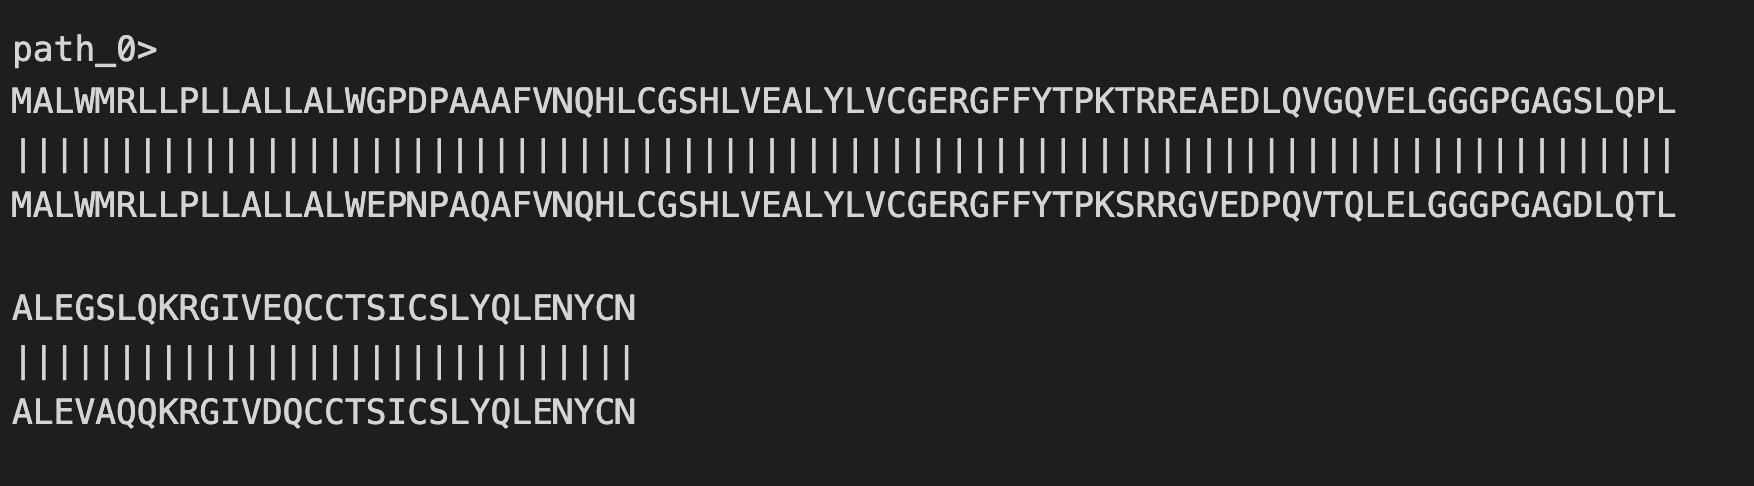
\includegraphics[scale=0.5]{sample.png}
\section{Methods}
\subsection{Needleman-Wunsch algorithm}
Needleman-Wunsch Algorithm is a method to find the optimal alignment with
the highest score. \\
The Needleman-Wunsch Algorithm is based on dynamic programming.\\
We use a Score Matrix to calculate the optimal score and a corresponding Array Matrix for returning the optimal alignment path. \\
score[i][j] represents the optimal score for the (sub) global alignment $X_i',Y_j'$ of two sub-sequences
\[
    X_i = (x_1, ..., x_i)
\]
and
\[
    Y_i = (y_1, ..., y_j)
\]
which start from $x_1$, $y_1$ and end with $x_i$ and $y_j$. \\
The (sub) global alignment $X_i',Y_j'$ of sub-sequences $X_i, Y_j$ can be calculated from former positions in at most 3 situations: \\
1. Add both $x_i$ and $y_j$ to the ends of $X_{i-1}'$ and $Y_{j-1}'$; \\
\indent In this case, the delta score depends on if $x_i = y_j$.\\
2. Keep $X_i' = X_{i-1}'$ but add $y_j$ to the end of $Y_{j-1}'$; \\
\indent In this case, the delta score will be the gap punishing score.\\
3. Keep $Y_i' = Y_{i-1}'$ but add $x_j$ to the end of $X_{j-1}'$; \\
\indent In this case, the delta score will be the gap punishing score.\\
In each step, we choose the maximum score from the 3 options, and update the Score Matrix. \\
The $X_0'$ and $Y_0'$ are set to empty strings at the beginning.\\
If the score is one of the best one(s), we set an arrow into the arrow matrix for retrieving the optimal path.
\subsection{Score Matrix}
\paragraph{Initialization} 
For (0, 0) we set score[0][0] = 0.
\paragraph{DP State Transition Function}
\[
    score[i][j] = Max 
    \begin{cases}
        score[i-1, j-1] + F(x'_i, y'_j); \quad & \text{ if } i-1>=0 \text{ and } j-1>=0, \\
        score[i-1, j] + F(x'_i, \text{'-'}); \quad & \text{ if } i-1>=0, \\
        score[i, j-1] + F(\text{'-'}, y'_j); \quad & \text{ if } j-1>=0,  \\
    \end{cases}
\]
\paragraph{The Global Optimal Score}
score[m, n] is the global optimal score because in this case the subsequences are the sequences themselves.
\subsection{Arrow Matrix}
If the score is one of the best one(s), we set an arrow into the arrow matrix for retrieving the optimal path.
\begin{itemize}
    \item if $score[i][j] = score[i-1, j-1] + F(x'_i, y'_j)$, we set arrow from (i, j) to (i-1, j-1);
    \item if $score[i][j] = score[i-1, j] + F(x'_i, '-')$, we set arrow from (i, j) to (i-1, j);
    \item if $score[i][j] = score[i, j-1] + F('-', y'_j)$, we set arrow from (i, j) to (i, j-1)
\end{itemize}
After calculating the whole matrix, we retrive the optimal path from the last cell [m, n] using Deep First Search towards [0,0] until we have found enough optimal paths. 
\section{Results}
\subsection*{Homologous genes alignment}
seq1: NM\_033034.3\\
Homo sapiens tripartite motif containing 5 (TRIM5), transcript variant alpha, mRNA\\
seq2: NM\_001032910.1\\
Macaca mulatta tripartite motif containing 5 (TRIM5), mRNA\\
\\
1. match=2, mismatch=-1, gap=0\\
best\_score: 5666.0\\
2. match=2, mismatch=-1, gap=-2.5\\
best\_score: 4511.0\\
\subsection*{Human and hamster insulin protein alignment}
seq1: AAA59172.1 insulin [Homo sapiens]\\
MALWMRLLPLLALLALWGPDPAAAFVNQHLCGSHLVEALYLVCGERGFFYTPKTRREAEDLQVGQVELGG
GPGAGSLQPLALEGSLQKRGIVEQCCTSICSLYQLENYCN\\
seq2: XP\_003508128.1 insulin [Cricetulus griseus]\\
MALWMRLLPLLALLALWEPNPAQAFVNQHLCGSHLVEALYLVCGERGFFYTPKSRRGVEDPQVTQLELGG
GPGAGDLQTLALEVAQQKRGIVDQCCTSICSLYQLENYCN\\
\\
1. match=2, mismatch=-1, gap=0\\
best\_score: 190.0\\
2. match=2, mismatch=-1, gap=-2.5\\
best\_score: 175.0\\
\section{Discussion}
1. The complexity of this 2-dimensional dynamic programming algorithm is $O(n^2)$. \\
However, the complexity of retrieving all the optimal paths depends on the number P of elements that have multiple arrows and brings an exponentially increasing complexity $O(2^P)$. \\
To control the total time complexity, we use a parameter maximum\_size to restrict the number of returning paths. We do the Deep First Search until we have found maximum\_size paths.\\
2. We can represent arrow using a integer flag using bit-encode:\\
arrow to (i-1, j-1): flag += 1;\\
arrow to (i-1, j): flag += 2;\\
arrow to (i, j-1): flag += 4\\
so we can get:\\
if flag \& 1: there is an arrow from (i,j) to (i-1, j-1);\\
if flag \& 2: there is an arrow from (i,j) to (i-1, j);\\
if flag \& 4: there is an arrow from (i,j) to (i, j-1)\\
3. In the experiments, two Score Functions are used. One of them punishes gapping stronger than mismatching, and the other does not punish gapping(score=0). 0 is the maximum score we can give gapping, because a positive score will give bonus to the bahavior of dropping the matching for prelonging the alignment sequences.
\section{Conclusion}
We implement the Needleman-Wunsch Algorithm for global sequence alignment and retrieve multiple optimal paths using Deep First Search. \\We test it on 2 datasets for aligning nucleotide sequences or amino acid sequences. \\We also test the effects of different scoring functions, which control the preferences for mismatching or gapping.
\bibliography{refs}
\end{document}